\setlength{\fboxrule}{2pt}
\newcommand\fboxg{\fcolorbox{green}{white}}
\newcommand\fboxr{\fcolorbox{red}{white}}
\renewcommand{\imglabel}[1]{\put(2,5){\small\contour{black}{\textcolor{white}{\textbf{#1}}}}}
\begin{figure}[h]
	\centering
	\setlength{\resLen}{0.2\columnwidth}	
	\addtolength{\tabcolsep}{0pt}
	\begin{tabular}{cccc}
		Photo & \textit{Leather} Prior & \textit{Plaster} Prior & \textit{Wood} Prior
		\\
		\begin{overpic}[width=\resLen]{bayesian/fig7/2_leather_5/target.jpg}
			\imglabel{Leather-5}
		\end{overpic} &
		\fboxg{\includegraphics[width=\resLen]{bayesian/fig7/2_leather_5/good1.jpg}} &
		\fboxr{\includegraphics[width=\resLen]{bayesian/fig8/2_leather_5/plaster.jpg}} &
		\fboxr{
\includegraphics[width=\resLen]{bayesian/fig8/2_leather_5/wood.jpg}} 
		\\[5pt]
		\begin{overpic}[width=\resLen]{bayesian/fig7/6_wood_5/target.jpg}
			\imglabel{Wood-5}
		\end{overpic} &
		\fboxr{
\includegraphics[width=\resLen]{bayesian/fig8/6_wood_5/leather.jpg}} &
		\fboxr{\includegraphics[width=\resLen]{bayesian/fig8/6_wood_5/plaster.jpg}} &
		\fboxg{\includegraphics[width=\resLen]{bayesian/fig7/6_wood_5/good1.jpg}} 
	\end{tabular}
	\caption[Comparison with mismatched model]{\label{fig:bayesian:mismatch}
		\textbf{Comparison} with mismatched forward models. With an inappropriate model as the prior, it would only match the global color but missing all the details.   
	}
\end{figure}